%% 
%% Copyright 2007-2019 Elsevier Ltd
%% 
%% This file is part of the 'Elsarticle Bundle'.
%% ---------------------------------------------
%% 
%% It may be distributed under the conditions of the LaTeX Project Public
%% License, either version 1.2 of this license or (at your option) any
%% later version.  The latest version of this license is in
%%    http://www.latex-project.org/lppl.txt
%% and version 1.2 or later is part of all distributions of LaTeX
%% version 1999/12/01 or later.
%% 
%% The list of all files belonging to the 'Elsarticle Bundle' is
%% given in the file `manifest.txt'.
%% 

%% Template article for Elsevier's document class `elsarticle'
%% with numbered style bibliographic references
%% SP 2008/03/01
%%
%% 
%%
%% $Id: elsarticle-template-num.tex 168 2019-02-25 07:15:41Z apu.v $
%%
%%
\documentclass[preprint,12pt]{elsarticle}

%% Use the option review to obtain double line spacing
%% \documentclass[authoryear,preprint,review,12pt]{elsarticle}

%% Use the options 1p,twocolumn; 3p; 3p,twocolumn; 5p; or 5p,twocolumn
%% for a journal layout:
%% \documentclass[final,1p,times]{elsarticle}
%% \documentclass[final,1p,times,twocolumn]{elsarticle}
%% \documentclass[final,3p,times]{elsarticle}
%% \documentclass[final,3p,times,twocolumn]{elsarticle}
%% \documentclass[final,5p,times]{elsarticle}
%% \documentclass[final,5p,times,twocolumn]{elsarticle}

%% For including figures, graphicx.sty has been loaded in
%% elsarticle.cls. If you prefer to use the old commands
%% please give \usepackage{epsfig}

%% The amssymb package provides various useful mathematical symbols
\usepackage{amssymb}
\usepackage{amsmath}
%% The amsthm package provides extended theorem environments
\usepackage{amsthm}

\newtheorem{theorem}{Theorem}


%% The lineno packages adds line numbers. Start line numbering with
%% \begin{linenumbers}, end it with \end{linenumbers}. Or switch it on
%% for the whole article with \linenumbers.
%% \usepackage{lineno}

\journal{Discrete Mathematics}

\begin{document}

\begin{frontmatter}

%% Title, authors and addresses

%% use the tnoteref command within \title for footnotes;
%% use the tnotetext command for theassociated footnote;
%% use the fnref command within \author or \address for footnotes;
%% use the fntext command for theassociated footnote;
%% use the corref command within \author for corresponding author footnotes;
%% use the cortext command for theassociated footnote;
%% use the ead command for the email address,
%% and the form \ead[url] for the home page:
%% \title{Title\tnoteref{label1}}
%% \tnotetext[label1]{}
%% \author{Name\corref{cor1}\fnref{label2}}
%% \ead{email address}
%% \ead[url]{home page}
%% \fntext[label2]{}
 \cortext[cor1]{Corresponding Author.}
 \fntext[fn1]{This work was supported by National Science Foundation grant \#ECCS-2013779.}
%% \address{Address\fnref{label3}}
%% \fntext[label3]{}

\title{An Upper Bound on the Cardinality of a Minimum Feedback Vertex Set for Directed Graphs}

%% use optional labels to link authors explicitly to addresses:
%% \author[label1,label2]{}
%% \address[label1]{}
%% \address[label2]{}

\author{Philip N. Brown\corref{cor1}%
\fnref{fn1}}


\address{Department of Computer Science\\ University of Colorado Colorado Springs\\ USA 80918}

\begin{abstract}
We derive an upper bound on the cardinality of a minimum feedback vertex set for arbitrary directed graphs, and provide example graphs which achieve this bound.
\end{abstract}


%%Research highlights
%\begin{highlights}
%\item Research highlight 1
%\item Research highlight 2
%\end{highlights}

\begin{keyword}
Directed Graphs \sep Combinatorics \sep Feedback Vertex Sets
%% keywords here, in the form: keyword \sep keyword

%% PACS codes here, in the form: \PACS code \sep code

%% MSC codes here, in the form: \MSC code \sep code
%% or \MSC[2008] code \sep code (2000 is the default)

\end{keyword}

\end{frontmatter}

%% \linenumbers

%% main text

Let $G=(V,E)$ be a directed, not necessarily connected graph.
%A \emph{directed cycle} in $G$ is a sequence of distinct vertices $\{e_1,\dots,e_i\}\subseteq E$ such that 
A subset of vertices $M\subseteq V$ is called a \emph{minimum feedback vertex set} if the subgraph induced by the removal of $M$ from $G$ contains no directed cycles and $M$ is the smallest such set of vertices.
The problem of finding a minimum feedback vertex set in an arbitrary graph is known to be NP-hard even in sparse graphs~\cite{Fomin2006,Borradaile2019} and its decision version was one of Karp's original 21 NP-complete problems~\cite{Karp1972}.
Nonetheless, identifying minimum feedback vertex sets in directed graphs has applications in a number of disparate domains, including deadlock recovery in operating systems and computer engineering~\cite{Lin2000}, and determining the inefficiency of Nash equilibria in game theory~\cite{Brown2019c}.


Recent years have seen considerable attention focused on deriving bounds on the cardinality of the minimum feedback vertex set for undirected graphs. For instance see bounds for planar graphs~\cite{Kelly2017}, hypercubes~\cite{Madelaine2008}, shuffles~\cite{Kralovic2003}, and further conjectures~\cite{Kowalik2010}.
However, there seems to be a lack of similar results for the valuable case of directed graphs.
Accordingly, this note presents a simple upper bound for this quantity for directed graphs as a function of the number of nodes and edges.
We present graphs that achieve this bound.
While tight in general, this bound can almost certainly be improved on specific classes of graphs, and we invite improvements from the mathematical community.

\section{Preliminaries}
We present the following definitions to ensure our results are clear.
A directed graph $G=(V,E)$ (or \emph{digraph}) is specified by vertex set $V$ and edge set $E$ and we assume that $G$ is simple (i.e., we forbid repeated edges or self-loops), but we do not require that $G$ is connected.
A \emph{directed cycle} is a sequence of distinct edges $\{e_1,e_2,\ldots,e_m\}$ and a corresponding sequence of distinct vertices $\{v_1,v_2,\ldots,v_m\}$ such that for all $i<m$, $e_i=(v_i,v_{i+1})$ and $e_m=(v_m,v_1)$.
Note that a directed cycle can have length 2; i.e., the graph $(\{v_1,v_2\},\{(v_1,v_2),(v_2,v_1)\})$ has a directed cycle.
A digraph $G$ is called \emph{acyclic} if if it contains no directed cycles.
A set of vertices $M\subseteq V$ is called a \emph{feedback vertex set} if the graph $\left(V\setminus M,E\setminus \{(i,j)\in E\ |\ i\in M \mbox{ or } j\in M\}\right)$ is acyclic.
The set $M$ is called a \emph{minimum feedback vertex set} if it is a feedback vertex set of minimum cardinality. 
We write $\alpha(G)$ to denote the cardinality of a minimum feedback vertex set for digraph $G$.

\section{Contribution}


Our main result gives a tight upper bound for all (not necessarily connected) digraphs as a function of the number of edges.
\begin{theorem}\label{thm:main}
Let $G=(V,E)$ be a digraph.
Then
\begin{equation}\label{eq:main}
\alpha(G) \leq \min\left\{|V|-1,\left\lfloor\frac{|E|}{2}\right\rfloor\right\}.
\end{equation}
There exist graphs which achieve this bound.
\end{theorem}

\begin{proof}
First we show the edge-based upper bound.
Let $G$ be a directed graph, and let $M(G)$ be a minimum feedback vertex set of $G$.
We wish to show that 
\begin{equation}
2\alpha(G)\leq |E|.
\end{equation}
Enumerate the $m$ vertices in $M(G):=\{u_1,u_2,\ldots,u_m\}$.
%Define $E(M(G)):=\{
Define the sequence $\{G_i\}_{i=0}^m$ as follows: $G_0=G$, and $G_i$ is the digraph that results from the removal of $u_i$ and all incident edges from $G_{i-1}$.
By the definition of $M(G)$, each vertex $u_i$ is contained in at least one cycle in graph $G_{i-1}$.
Since each $u_i$ is contained in a cycle in $G_{i-1}$, it follows that at least 2 edges are incident on $u_i$ in $G_{i-1}$.
Since the sequence of graphs satisfies $E(G_{i})\subset E(G_{i-1})$, this means that for all $i=1,\ldots,m$, at least 2 unique edges are incident on vertex $u_i$ which are \emph{not} incident on $u_j$ for any $j<i$.
%
Thus, writing $E(M(G))$ to denote the set of edges incident on $M(G)$, we have that
\begin{equation}
2\alpha(G)\leq|E(M(G))|\leq |E|.
\end{equation}

\begin{figure}[h]
\centering
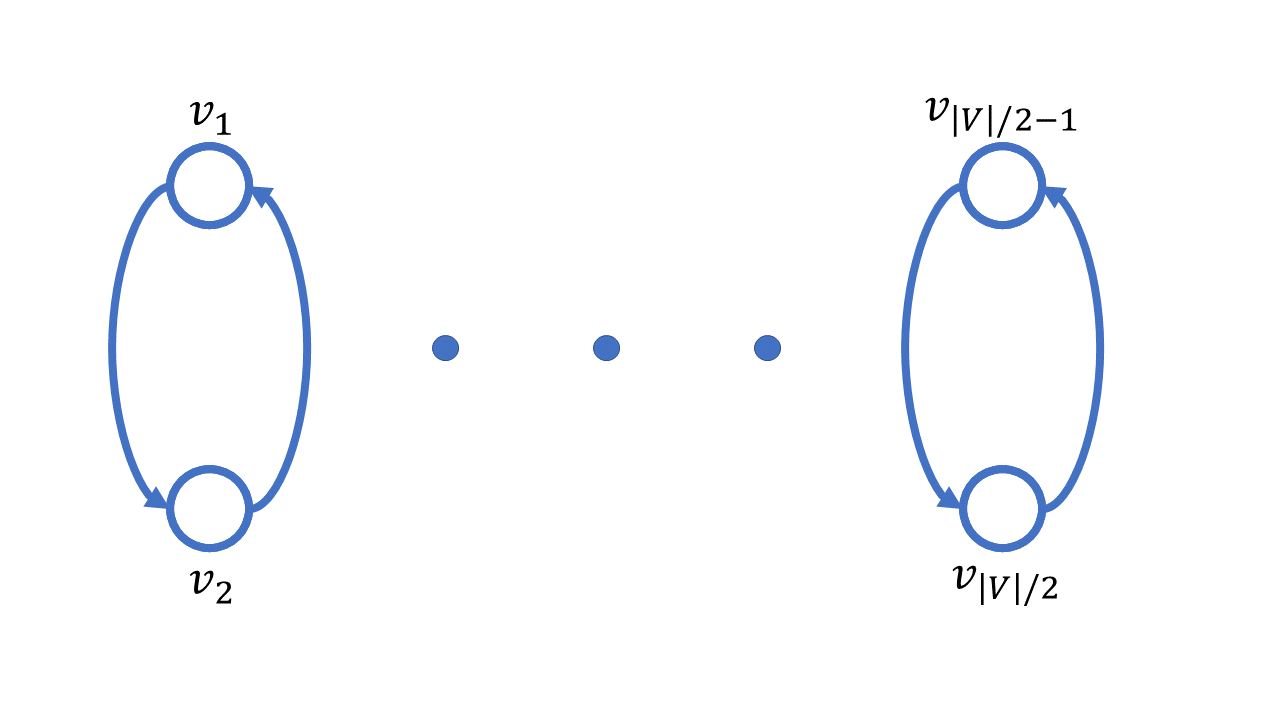
\includegraphics[width=.75\textwidth]{gfx/graph}
\caption{\label{fig:graph} Graph with $\alpha(G)=\lfloor|E|/2\rfloor$, achieving the bound given in Theorem~\ref{thm:main} in~\eqref{eq:main}.}
\end{figure}

To show the edge-based lower bound, we construct a family of graphs which satisfy~\eqref{eq:main} with equality for all $k$, where $|E|=k$.
Let $|V|=2\lfloor k/2\rfloor$, and let $E=\{(2i,2i-1)\cup(2i-1,2i)\ |\ i\in\{1,\ldots,|V|/2\}\}$ (see Figure~\ref{fig:graph}).
If $|E|$ is odd, define the single remaining edge between any feasible pair of vertices (e.g., $(1,3)$).
Since this graph contains exactly $|V|/2$ disjoint length-2 directed cycles, the cardinality of any minimum feedback vertex set is exactly $|V|/2$ (e.g., the set of odd-numbered vertices is such a set).
%


The vertex-based upper bound is trivial, since if $|V|-1$ vertices and associated edges are removed from any graph, the resulting graph is a single vertex and thus acyclic.
The vertex-based lower bound is achieved by a complete digraph.
\end{proof}



%% The Appendices part is started with the command \appendix;
%% appendix sections are then done as normal sections
%% \appendix

%% \section{}
%% \label{}

%% If you have bibdatabase file and want bibtex to generate the
%% bibitems, please use
%%
\bibliographystyle{elsarticle-num} 
\bibliography{../../library/library}

\end{document}
\endinput
%%
%% End of file `elsarticle-template-num.tex'.
